\section{Internet Layer}


\subsection{IPv4}

\subsubsection{Header}

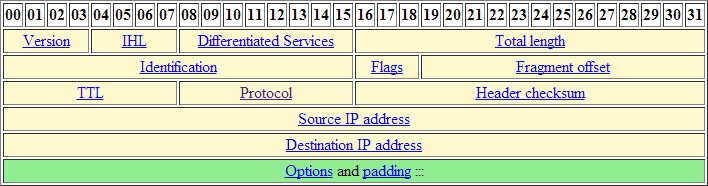
\includegraphics[width=\textwidth]{media/ipv4_header.png}

\subsubsection{Ports}

\begin{tabular}[h]{|l|l|}
	\hline
  \textbf{Range} & \textbf{Description} \\
	\hline
  0--1023 & Well known Ports \\
  1024--49151 & Registered Ports\\
  49152--65535 & Ephemeral Ports\\
	\hline
\end{tabular}

Wenn eine TCP Verbindung geschlossen wird, verbleibt der Port für eine
festgelegte Zeit (üblicherweise ca 120s) im Status TIME\_WAIT und kann in dieser
Zeit nicht wiederverwendet werden.

\subsubsection{Protocol}

\begin{tabular}[h]{|l|l|}
	\hline
  \textbf{Value} & \textbf{Protocol} \\
	\hline
  1 & ICMP \\
  6 & TCP \\
  17 & UDP \\
  41 & IPv6 over IPv4 \\
	\hline
\end{tabular}


\subsection{IPv6}

\subsubsection{Header}

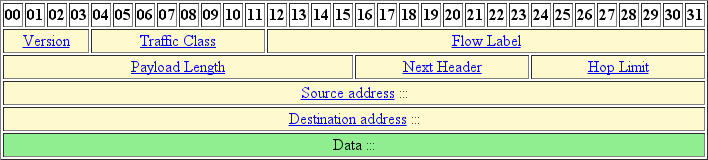
\includegraphics[width=\textwidth]{media/ipv6_header.png}

\subsubsection{Adressbildung}

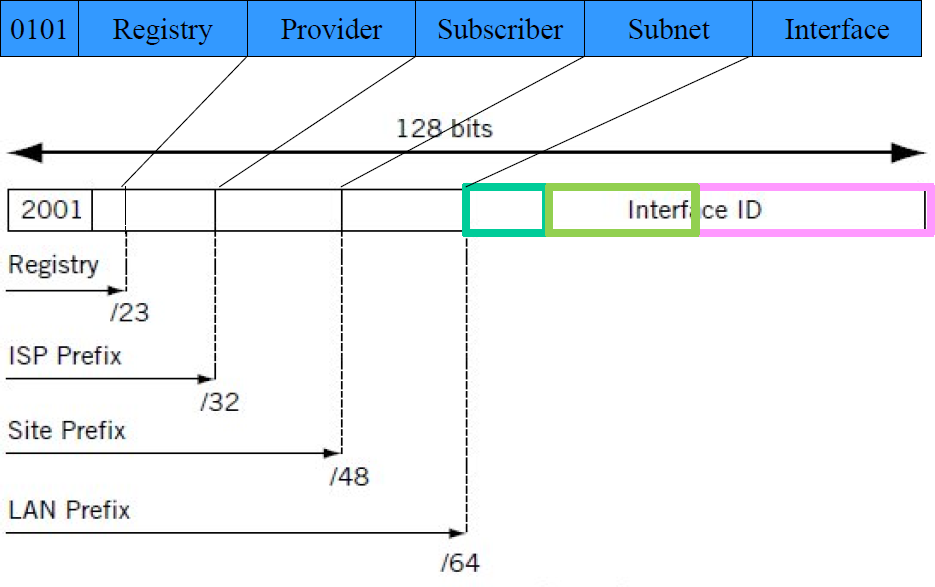
\includegraphics[width=\textwidth]{media/ipv6.png}

Präfix + Netzwerkstruktur + Interface-Identifier = 128Bit IPV6 Adresse\\
Prefix + Netzwerkstruktur = 64Bit\\
Interface-Identifier = 3Byte MAC OUI + ff:fe + 3Byte MAC NIC\\
Wobei im MAC OUI Teil das globally administered bit (7bit, $2^{2}$ Position) gesetzt wird.

Beispiel MAC: 58:55:ca:f3:e1:29Y\\
1. ff:fe einfügen: 58:55:ca:ff:fe:f3:e1:29\\
2. Globally administered Bit setzten: 58 = 01010100 => 01010110, 5a\\
3. Resultierende Adresse: 5a55:caff:fef3:e129

\textbf{Vereinfachungen}

\begin{itemize}
	\item Führende Nullen innerhalb eines Blockes dürfen ausgelassen werden.
	\item Ein oder mehrere aufeinander folgende Blöcke, deren Wert 0 (bzw. 0000)
		beträgt, dürfen ausgelassen werden. Dies wird durch zwei aufeinander
		folgende Doppelpunkte angezeigt.
	\item Die Reduktion durch Regel 3 darf nur einmal durchgeführt werden, das
		heisst, es darf höchstens eine zusammenhängende Gruppe aus Null-Blöcken in
		der Adresse ersetzt werden. Die Adresse 2001:0db8:0:0:8d3:0:0:0 darf demnach
		entweder zu 2001:db8:0:0:8d3:: oder 2001:db8::8d3:0:0:0 gekürzt werden;
		2001:db8::8d3:: ist unzulässig, da dies mehrdeutig ist und fälschlicherweise
		z.B. auch als 2001:db8:0:0:0:8d3:0:0 interpretiert werden könnte.
	\item Ebenfalls darf für die letzten vier Bytes (also 32 Bits) der Adresse die
		herkömmliche dezimale Notation verwendet werden. So ist ::ffff:127.0.0.1
		eine alternative Schreibweise für ::ffff:7f00:1. Diese Schreibweise wird vor
		allem bei Einbettung des IPv4-Adressraums in den IPv6-Adressraum verwendet.
	\item Beispiel: 2001:0db8:0:0:0:0:7f00:0001 ist gleichbedeutend mit
		2001:db8::127.0.0.1.
\end{itemize}

\subsubsection{Besondere Adressen}

In IPv6 gibt es sehr viele spezielle Adressen und Adressbereiche, speziell bei
Multicast. Hier ein Auszug davon:

\begin{tabular}[h]{|l|l|l|}
	\hline
	\textbf{Address} & \textbf{Type} & \textbf{Description} \\
	\hline
	::/0 & Default Route & Default Route (IPv4: 0.0.0.0/0) \\
	::1/128 & Local & Loopback (IPv4: 127.0.0.0/8) \\
	fe80::/10 & Local & Link Local Addresses (IPv4: 169.254.0.0/16) \\
	::/0 & Local & Unique Local Addresses (IPv4: Private Address Ranges) \\
	ff00::/8 & Multicast & Multicast Range \\
	ff0X::1 & Multicast & All Nodes (Scopes 1, 2) \\
	ff0X::2 & Multicast & All Routers (Scopes 1, 2, 3) \\
	ff02::1:2 & Multicast & All DHCP Agents \\
	ff05::1:3 & Multicast & All DHCP Servers \\
	\hline
\end{tabular}

In den Multicast-Adressen steht das X für den Scope. Verfügbare Scopes:

\begin{tabular}[h]{|l|l|}
	\hline
	\textbf{Value} & \textbf{Description} \\
	\hline
	1 & interface-local \\
	2 & link-local \\
	5 & site-local \\
	\hline
\end{tabular}


\subsection{ICMP}

\subsubsection{Header}

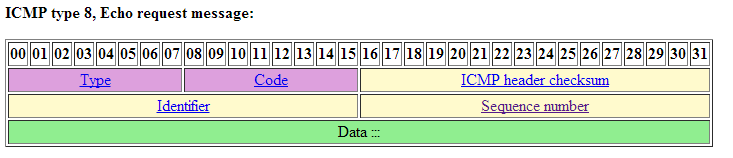
\includegraphics[width=\textwidth]{media/ICMPRequest.png}

\subsubsection{NAT/PAT}

Da ICMP Pakete keine Ports kennen, muss ein Router seine PAT Tabelle anders
realisieren. Er verwendet dazu die Sequenznummern der Echo/Reply Pakete. Die Sequenznummern
dienen dazu, eine Antwort einem Request zuzuweisen. Ein Implementationsvariante
ist, dass der Router anstelle des Ports die Sequenznummer verwendet, oder diese
einem virtuellen Port zuweist.
